% !TeX root = main.tex
\documentclass[11pt,oneside,a4paper]{article}

%%%%%%%%%%%%%%%%%%%%%%%%%%%%%%%%%%%%%%%%%%%%%%%%%%%%%%%%%%%%%%%%%%%%%%%
%					IMPOSTAZIONE TEMPLATE DOCUMENTO					  %
%%%%%%%%%%%%%%%%%%%%%%%%%%%%%%%%%%%%%%%%%%%%%%%%%%%%%%%%%%%%%%%%%%%%%%%

% !TeX root = ../main.tex
%%%%%%%%%%%%%%%%%%%%%%%%%%%%%%%%%%%%%%%%%%%%%%%%%%%%%%%%%%%%%%%%%%%%%%%
%                   IMPOSTAZIONE TEMPLATE DOCUMENTO                   %
%%%%%%%%%%%%%%%%%%%%%%%%%%%%%%%%%%%%%%%%%%%%%%%%%%%%%%%%%%%%%%%%%%%%%%%

\usepackage[english]{babel}        % Impostato su inglese
\usepackage[T1]{fontenc}
\usepackage{lmodern}
\usepackage{amsmath}       % per le formule delle sezioni PCA, LogReg e SVM
\usepackage{amssymb}       % \mathbb (es. \mathbb{R})
\usepackage[a-1b]{pdfx}    % per archiviazione pdfA
\usepackage[a4paper,margin=2cm,includeheadfoot,headheight=14pt,headsep=8pt,footskip=18pt]{geometry}
\usepackage{graphicx}      % \includegraphics
\usepackage{float}         % posizionamento [H]
\usepackage{booktabs}      % \toprule, \midrule, \bottomrule
\usepackage{tikz}          % schema della pipeline

\usepackage{fancyhdr}      % impaginazione
\pagestyle{fancy}
\fancyhf{}
\fancyhead{} % clear all header fields
\fancyhead[R]{\small\nouppercase{\rightmark}}
\fancyfoot{} % clear all footer fields
\fancyfoot[R]{\thepage}
\renewcommand{\sectionmark}[1]{\markright{\thesection\ #1}}
\renewcommand{\headrulewidth}{0.1pt}
\renewcommand{\footrulewidth}{0.1pt}
\usepackage[font={small,it},skip=4pt]{caption}

\linespread{1.0}\selectfont
\raggedbottom

\makeatletter  % per fare in stile FANCY tutte le pagine
\let\ps@plain=\ps@fancy
\makeatother

%%%%%%%%%%%%%%%%%%%%%%%%%%%%%%%%%%%

% Definitions
\def\texttilde{{\raise.17ex\hbox{$\scriptstyle\sim$}}}

% Paragraph Editor
\usepackage[parfill]{parskip}
\setlength{\parskip}{0.25em}
\setlength{\parindent}{0pt}

% Compact spacing around figures and tables.
\setlength{\textfloatsep}{8pt plus 2pt minus 2pt}
\setlength{\floatsep}{6pt plus 2pt minus 2pt}
\setlength{\intextsep}{6pt plus 2pt minus 2pt}
\setlength{\tabcolsep}{4pt}

%%%%%%%%%%%%%%%%%%%%%%%%%%%%%%%%%%%%
%Per inserire reference a link esterni
\usepackage{hyperref}
\hypersetup{hidelinks}

%%%%%%%%%%%%%%%%%%%%%%%%%%%%%%%%%%%%%
%includi stampe con print

\usepackage{xcolor}
\usepackage{listings}
\lstdefinestyle{out}{
    basicstyle=\ttfamily\small,
    backgroundcolor=\color{gray!10},
    frame=single,
    framerule=0pt,
    breaklines=true,
    xleftmargin=5pt,
    framexleftmargin=5pt
}

\usepackage{titlesec}
\titleformat{\section}{\normalfont\Large\bfseries}{\thesection}{0.6em}{}
\titleformat{\subsection}{\normalfont\large\bfseries}{\thesubsection}{0.6em}{}
\titleformat{\subsubsection}{\normalfont\normalsize\itshape}{\thesubsubsection}{0.6em}{}
\titlespacing*{\section}{0pt}{11pt plus 2pt minus 2pt}{5pt}
\titlespacing*{\subsection}{0pt}{7pt plus 1pt minus 1pt}{3pt}
\titlespacing*{\subsubsection}{0pt}{5pt plus 1pt minus 1pt}{2pt}


%%%%%%%%%%%%%%%%%%%%%%%%%%%%%%%%%%%%%%%%%%%%%%%%%%%%%%%%%%%%%%%%%%%%%%%
%						       	TITOLO 			    		  		  %
%%%%%%%%%%%%%%%%%%%%%%%%%%%%%%%%%%%%%%%%%%%%%%%%%%%%%%%%%%%%%%%%%%%%%%%
\begin{document}

    \pagenumbering{roman}

    % !TeX root = ../main.tex
\begin{titlepage}
    \begin{center}
        {\fontsize{20}{24}\selectfont\textsc{Delft University of Technology}\par}
        \rule[0.1cm]{\textwidth}{0.1mm}
        \rule[0.5cm]{\textwidth}{0.6mm}
        {\fontsize{14}{17}\selectfont\bfseries Faculty of Electrical Engineering, Mathematics and Computer Science\par}
        \vspace{0.3cm}
        {\fontsize{14}{17}\selectfont\bfseries Machine Learning for Electrical Engineering - EE4C12\par}
    \end{center}

    \vspace{15mm}

    \begin{center}
        {\fontsize{28}{34}\selectfont\bfseries ECG Classification for\\Arrhythmia Detection\par}
    \end{center}

    \vspace{0.8cm}
    \begin{center}
        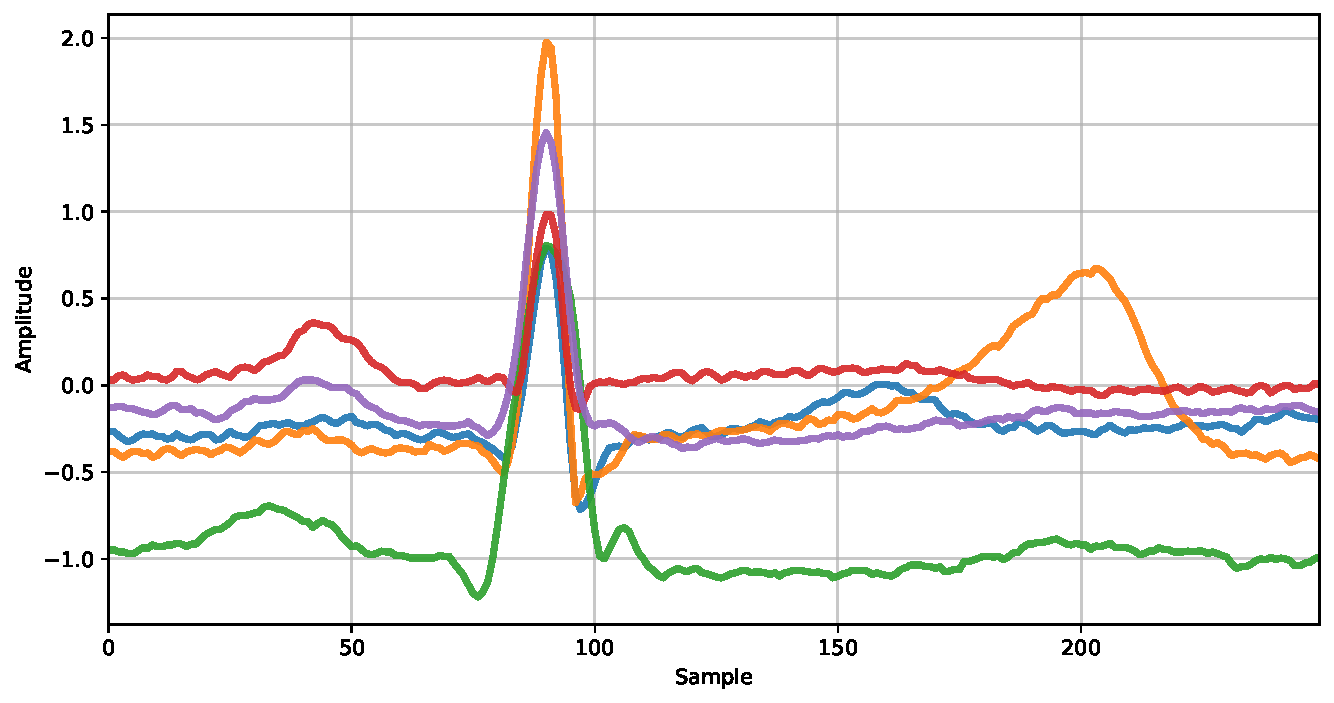
\includegraphics[width=\textwidth,height=7cm,keepaspectratio]{Images/ecg_heartbeats_cover.pdf}
    \end{center}

    \vfill

    \begin{center}
        {\fontsize{18}{22}\selectfont\bfseries Students}\\[0.5cm]

        \fontsize{13}{16}\selectfont
        \begin{tabular}{cc}
            Marco Bertazzoli Cova & Marco Fiorini
        \end{tabular}
    \end{center}
\end{titlepage}


    \clearpage
    \pagenumbering{arabic}



%%%%%%%%%%%%%%%%%%%%%%%%%%%%%%%%%%%%%%%%%%%%%%%%%%%%%%%%%%%%%%%%%%%%%%%
%								CAPITOLI 					  		  %
%%%%%%%%%%%%%%%%%%%%%%%%%%%%%%%%%%%%%%%%%%%%%%%%%%%%%%%%%%%%%%%%%%%%%%%

    \section*{Summary}
    This project addresses ECG heartbeat classification into the
    five AAMI classes required by the assignment. The resulting
    dataset is strongly imbalanced.

    We perform a data exploration procedure and we investigate normalization,
    standardization, PCA and FFT-based features. Trained models are selected using
    validation macro F1.
    The trained model families are logistic regression models, RBF SVM, fully connected neural
    networks and 1D convolutional neural networks.

    The best-performing model on the validation set is RBF-SVM,
    with a macro F1 of approximately 0.939. The best neural network architecture is the one
    with two hidden layers, 100 neurons each, trained on the raw data. This achieves a validation macro F1
    of 0.9375.

    An additional experiment is conducted: a neural network with the best found architecture is trained
    for classifying all the 15 classes. This experiment highlights the difficulty of recognizing classes
    with very few training examples.

    This project shows that greater architectural complexity does not necessarily improve performance.
    It also highlights the importance of evaluating minority classes alongside aggregate metrics.
    \section{Introduction and ML Pipeline}
    This project investigates ECG heartbeat classification into five
    AAMI classes and compares different machine learning approaches.
    The original labels are mapped to the AAMI groups, retaining the
    supplied training, validation and test splits. Preprocessing
    parameters and models are fitted using training data only.
    Preprocessing choices and hyperparameters are selected using
    validation macro F1. The selected SVM, MLP and CNN configurations are then evaluated
on the test set. Validation and test data
    receive the preprocessing transformations established during training,
    following the workflow discussed in the course~\cite{course_materials}.
    \begin{figure}[htbp]
        \centering
        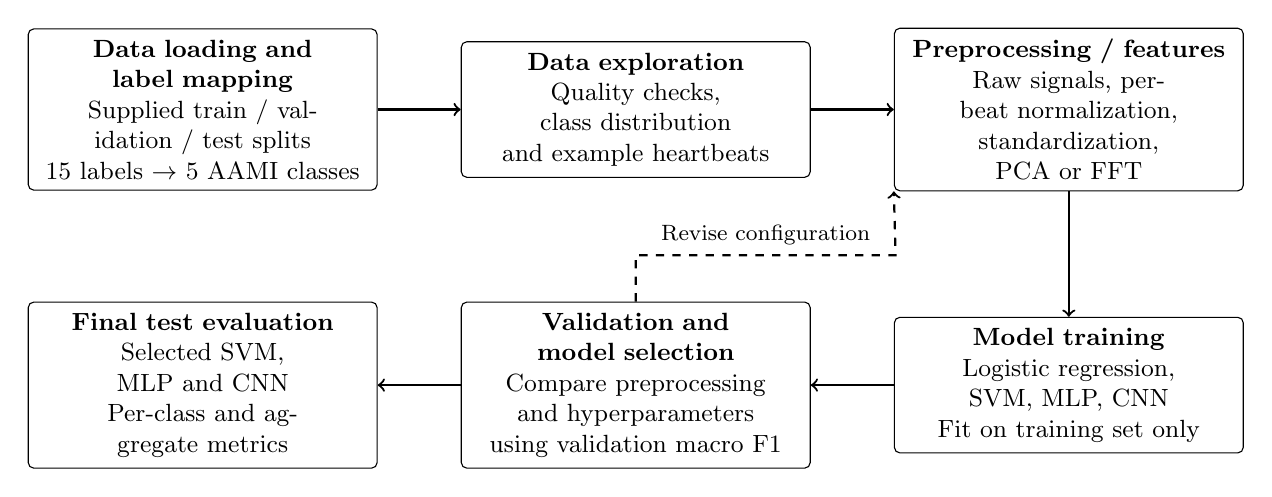
\begin{tikzpicture}[
            box/.style={
                draw,
                rounded corners=2pt,
                align=center,
                text width=4.15cm,
                minimum height=1.5cm,
                font=\small,
                inner sep=4pt
            },
            arrow/.style={->, thick}
        ]
            \node[box] (data) at (0,0)
                {\textbf{Data loading and label mapping}\\
                Supplied train / validation / test splits\\
                15 labels $\rightarrow$ 5 AAMI classes};

            \node[box] (analysis) at (5.5,0)
                {\textbf{Data exploration}\\
                Quality checks, class distribution\\
                and example heartbeats};

            \node[box] (prep) at (11,0)
                {\textbf{Preprocessing / features}\\
                Raw signals, per-beat normalization,\\
                standardization, PCA or FFT};

            \node[box] (model) at (11,-3.5)
                {\textbf{Model training}\\
                Logistic regression, SVM, MLP, CNN\\
                Fit on training set only};

            \node[box] (select) at (5.5,-3.5)
                {\textbf{Validation and model selection}\\
                Compare preprocessing and hyperparameters\\
                using validation macro F1};

            \node[box] (evaluate) at (0,-3.5)
                {\textbf{Final test evaluation}\\
                Selected SVM, MLP and CNN\\
                Per-class and aggregate metrics};

            \draw[arrow] (data.east) -- (analysis.west);
            \draw[arrow] (analysis.east) -- (prep.west);
            \draw[arrow] (prep.south) -- (model.north);
            \draw[arrow] (model.west) -- (select.east);
            \draw[arrow] (select.west) -- (evaluate.east);
            \draw[arrow, dashed] (select.north) -- (5.5,-1.85)
                -- node[above, font=\footnotesize]{Revise configuration}
                (8.8,-1.85) -- (prep.south west);
        \end{tikzpicture}

        \caption{Project workflow. Preprocessing and feature representations
        are alternatives or combinations compared during validation, rather
        than a mandatory sequence. Any fitted transformation uses training
        data only and is applied unchanged to validation and test data.
        Dashed arrows indicate tuning; the test set is used after selection.}
        \label{fig:classification_workflow}
    \end{figure}
    \section{Task 1: Data Analysis and Feature Engineering}
    \subsection{Data exploration}
    The supplied CSV files already contain segmented ECG heartbeats.
    Each row consists of 250 signal samples and one label identifying
    one of 15 original heartbeat types. The fixed splits contain
    65,670 training beats, 21,891 validation beats and 21,891 test beats,
    approximately corresponding to a 60/20/20 split. Quality checks
    found no missing or infinite values in the training data.

    The original labels are grouped into five AAMI classes, as reported
    in Table~\ref{tab:aami_classes}. The resulting dataset remains
    strongly imbalanced: N accounts for 82.77\% of training beats,
    whereas F accounts for only 0.73\%. Always predicting N would
    therefore achieve 82.77\% training accuracy without recognizing
    any minority class. This motivates per-class and macro-averaged
    evaluation.

    \begin{table}[htbp]
        \centering
        \begin{tabular}{llrr}
            \toprule
            AAMI class & Original beat types & Training beats & Share \\
            \midrule
            N & N, L, R, e, j & 54\,355 & 82.77\% \\
            S & A, a, J, S    & 1\,669  & 2.54\%  \\
            V & E, V         & 4\,341  & 6.61\%  \\
            F & F            & 481     & 0.73\%  \\
            Q & /, f, Q      & 4\,824  & 7.35\%  \\
            \bottomrule
        \end{tabular}
        \caption{AAMI mapping and training-set class distribution.}
        \label{tab:aami_classes}
    \end{table}

    Some original types are particularly rare. Original label 9
    (type S) has only two training examples and none in validation or
    test, preventing evaluation of its generalization performance
    in the 15-class experiment.

    Figure~\ref{fig:heartbeat_examples} illustrates variations in
    baseline, amplitude and waveform shape within and between
    heartbeat types. These observations motivate investigating
    normalization and alternative feature representations.

    \begin{figure}[htbp]
        \centering
        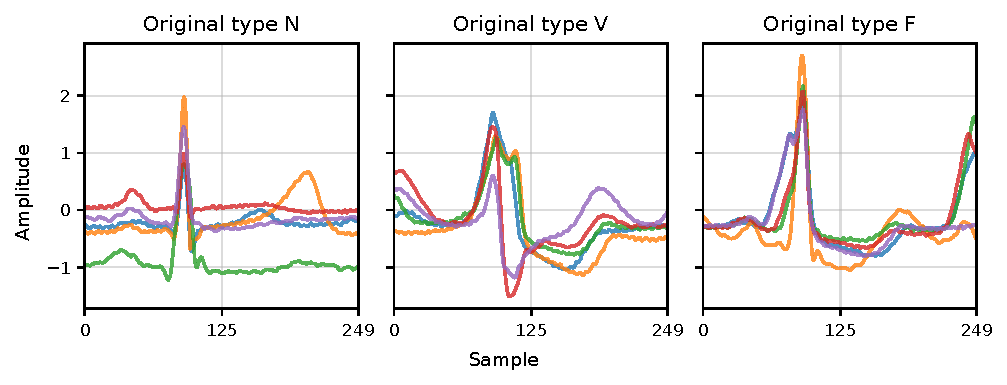
\includegraphics[width=0.95\linewidth]
            {Images/data_exploration_heartbeats.pdf}
        \caption{The first five training heartbeats from each original
        type N, V and F, plotted on common axes. These examples
        illustrate variability and do not represent the full
        distribution of each type.}
        \label{fig:heartbeat_examples}
    \end{figure}
    \subsection{Preprocessing methods}
    Since the supplied heartbeats are already segmented, we focus
    on scaling and feature representations. We compare per-beat
    normalization, standardization, PCA and FFT, assessing their
    usefulness through validation performance.
    \subsection{Standardization}
    All raw features are amplitude samples of the same ECG signal
    and therefore share a common measurement scale. Standardization
    was nevertheless tested to assess whether rescaling each input
    position could improve classification.

    We applied standardization using
    \texttt{StandardScaler}~\cite{sklearn_docs}. The scaler is fitted on the training set and
    reused for validation and test data. For the tested two-layer MLP,
    standardization did not improve validation macro F1: it decreased
    from 0.9375 on raw signals to 0.9301 on standardized signals.

    For logistic regression and SVM, we also tested per-beat
    normalization: each heartbeat is centered by subtracting its
    median and scaled by its standard deviation.
    \subsection{PCA analysis and dimensionality reduction}

    The 250 input features are correlated samples of the same
    heartbeat. PCA exploits this redundancy to reduce dimensionality,
    but preserving variance does not necessarily preserve features
    useful for classification. We examined cumulative explained
    variance, component shapes and per-class reconstruction errors
    to inform the choice of the number of retained components $k$.

    \subsubsection{Cumulative explained variance}
    PCA was fitted on raw training signals.
    Figure~\ref{fig:pca_variance} shows that 5, 8 and 17 components
    retain 90\%, 95\% and over 99\% of the variance, respectively.
    The first component alone explains 51.8\%.
    \begin{figure}[htbp]
        \centering
        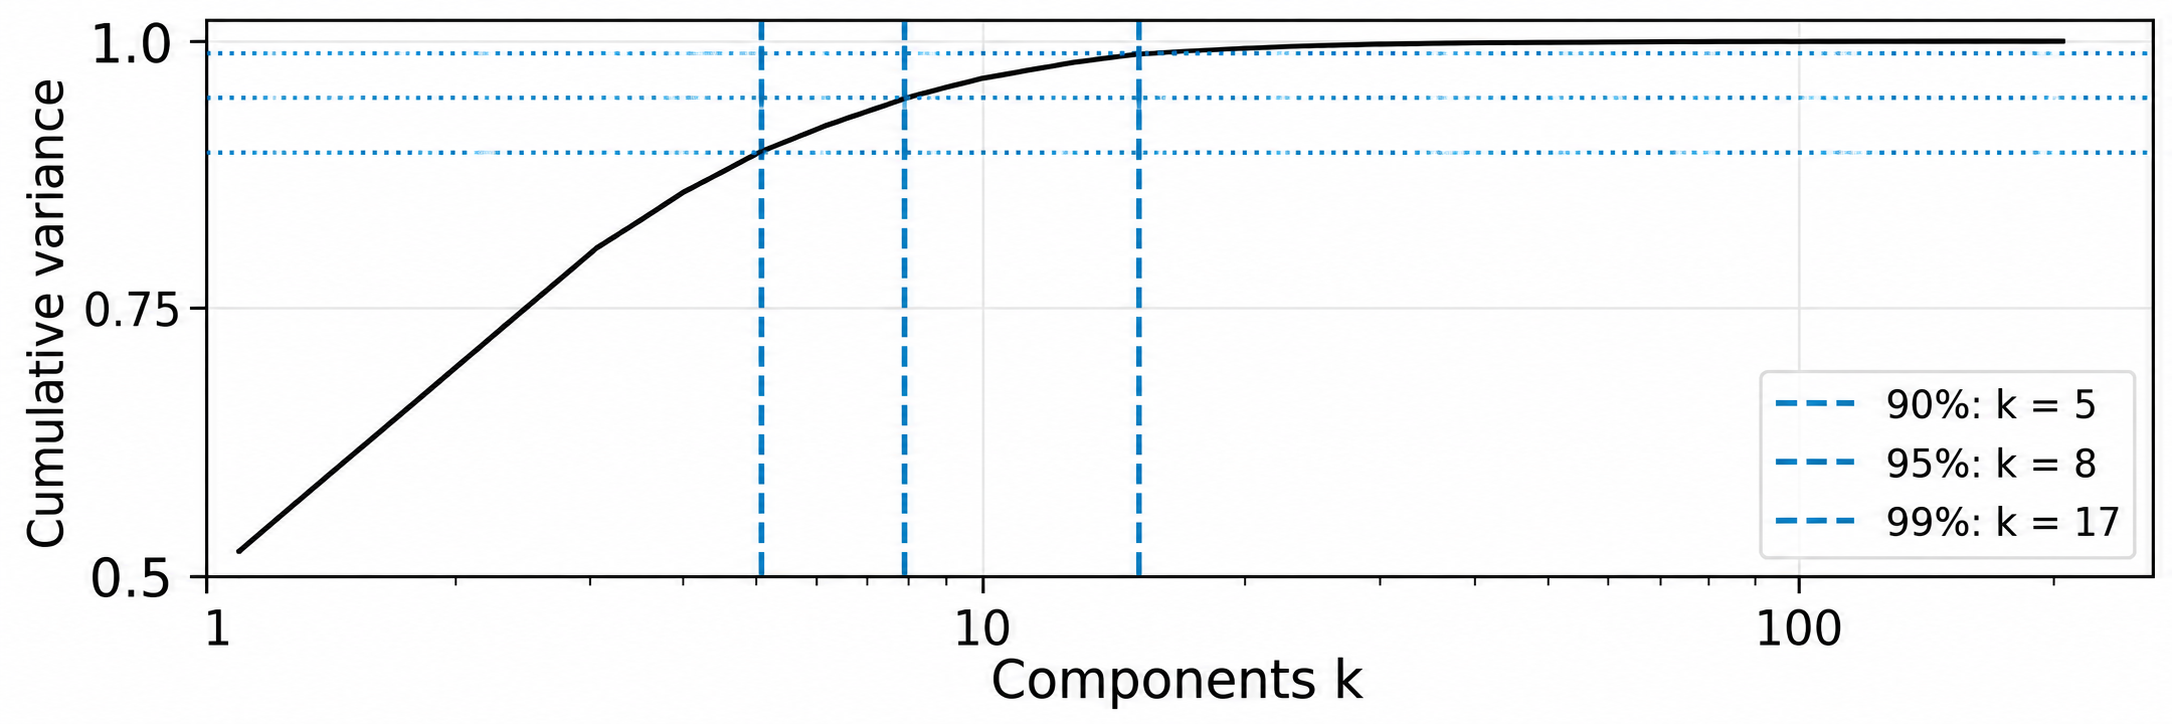
\includegraphics[width=0.65\linewidth]
            {Images/PCA_analysis/pca_explained_variance_compact.png}
        \caption{Cumulative explained variance of PCA fitted on the
        training set.}
        \label{fig:pca_variance}
    \end{figure}

    Although this result looks very promising, it does not mean
    that the remaining 1\% of the variance is irrelevant. As noted
    above, the variance is dominated by normal beats, so the
    discarded components may contain exactly the details that
    distinguish the minority classes. This is investigated in
    Section~\ref{sec:pca_reconstruction}.

    \subsubsection{Shape of the principal components}
    Each principal component is a vector of 250 weights, one for
    each time sample. It can therefore be plotted as a waveform
    and compared with the shape of a heartbeat.
    Figure~\ref{fig:pca_components} shows the first six components
    and the last three.

    \begin{figure}[htbp]
        \centering
        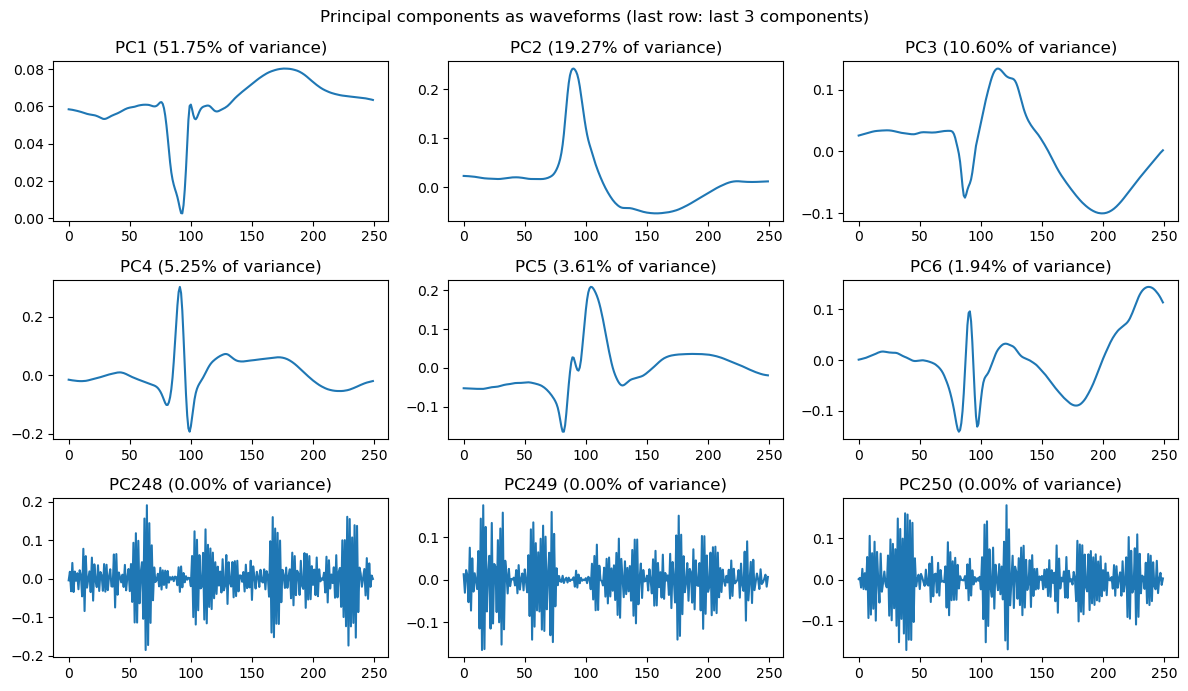
\includegraphics[width=\linewidth]
            {Images/PCA_analysis/pca_plot_components.png}
        \caption{First six and last three principal components of
        the training set, plotted as waveforms over the 250 samples.}
        \label{fig:pca_components}
    \end{figure}

    The first components are smooth and resemble parts of an ECG
    beat. The last components explain very little variance and
    show rapid oscillations. These may reflect noise or fine-scale
    signal details; their appearance alone does not establish
    whether they are useful for classification.

    \subsubsection{Per-class reconstruction error}
    \label{sec:pca_reconstruction}

    To measure how much information is lost when only the first
    $k$ components are kept, each beat $\mathbf{x}_i$ is projected
    onto these components and mapped back to the original 250
    samples:
    \begin{equation}
        \hat{\mathbf{x}}_i = \boldsymbol{\mu}
        + \mathbf{W}_k \mathbf{W}_k^{\top}
        (\mathbf{x}_i - \boldsymbol{\mu}),
    \end{equation}
    where $\boldsymbol{\mu}$ is the mean training beat and
    $\mathbf{W}_k \in \mathbb{R}^{250 \times k}$ contains the first
    $k$ principal components as columns. The reconstruction error
    of a beat is the mean squared difference between the original
    and the reconstructed signal:
    \begin{equation}
        e_i(k) = \frac{1}{250} \sum_{j=1}^{250}
        \left( x_{ij} - \hat{x}_{ij} \right)^2 .
    \end{equation}
    The errors are then averaged over the beats of each class $c$,
    giving $E_c(k)$. To compare the classes, we divide each value
    by the error of N, obtaining the relative error
    $R_c(k) = E_c(k) / E_N(k)$. A value of $R_c(k) = 3$ means that
    beats of class $c$ are reconstructed three times worse than
    normal beats. PCA is fitted on the training set, and the
    errors are computed on the validation set.

    The results are reported in Table~\ref{tab:pca_reconstruction}.
    With $k = 17$, which retains 99\% of the variance
    (Figure~\ref{fig:pca_variance}), S, V and Q are reconstructed
    about 2.7--2.8 times worse than N, and F about 1.9 times worse. 
    These differences indicate uneven reconstruction across classes,
    but do not directly measure the classification value of discarded
    components.

    \begin{table}[htbp]
        \centering
        \begin{tabular}{rrrrrr}
            \toprule
            $k$ & N & S & V & F & Q \\
            \midrule
            5   & 1.00 & 1.03 & 2.92 & 3.15 & 1.33 \\
            8   & 1.00 & 1.53 & 3.81 & 3.82 & 1.61 \\
            17  & 1.00 & 2.78 & 2.80 & 1.88 & 2.68 \\
            50  & 1.00 & 1.19 & 1.57 & 0.75 & 2.52 \\
            70  & 1.00 & 0.95 & 1.35 & 0.77 & 2.52 \\
            100 & 1.00 & 0.89 & 1.14 & 0.81 & 1.59 \\
            115 & 1.00 & 0.92 & 1.09 & 0.87 & 1.22 \\
            \bottomrule
        \end{tabular}
        \caption{Relative reconstruction error
        $R_c(k) = E_c(k)/E_N(k)$ of each class on the validation
        set, for different numbers of components $k$. Values are
        scaled on N, so the N column is always 1.}
        \label{tab:pca_reconstruction}
    \end{table}

    As $k$ increases, the relative errors approach 1. From
    $k = 50$, S and F are reconstructed about as well as N and
    V is within a factor of 1.6, while Q still has a relative
    error of about 2.5. Only around
    $k = 100$ are all the classes within a factor of 1.6 of N.

    With 100 components, reconstruction errors relative to N are
    closer to one, while dimensionality is reduced by 60\%.
    However, reconstruction quality does not determine the number
    of components required for classification. For example, the
    MLP using 17 raw-signal PCA components achieved validation
    macro F1 of 0.9310, compared with 0.9375 on raw signals.
    The usefulness of PCA must therefore be assessed for each
    classifier using validation performance.

    \subsection{FFT-based feature representation}

    We investigated frequency-domain features as an alternative
    to the raw amplitude samples. Applying \texttt{np.fft.rfft}
    to each heartbeat produces 126 complex coefficients.
    We tested two representations: concatenating their real and
    imaginary parts, yielding 252 features, and retaining only
    their magnitudes, yielding 126 features.
    \begin{lstlisting}[language=Python,
                    basicstyle=\ttfamily\footnotesize,
                    breaklines=true]
    spectrum = np.fft.rfft(X_train, axis=1)
    # Real and imaginary parts: 252 features
    X_train_fft = np.concatenate((spectrum.real, spectrum.imag), axis=1)
    # Magnitudes only: 126 features
    X_train_fft_mag = np.abs(spectrum)
    \end{lstlisting}
    Both representations were evaluated using the same MLP
    configuration, with two hidden layers of 100 neurons.
    Real and imaginary features achieved a validation macro F1
    of 0.9373, close to the 0.9375 obtained on raw signals.
    Standardizing these features reduced the score to 0.9025.

    Magnitude-only features reduced the input dimensionality
    by 49.6\% compared with raw signals, but achieved a lower
    macro F1 of 0.9113. This representation discards phase
    information, which may contribute to the performance loss.
    The raw-signal model therefore remained the preferred MLP
    configuration.
    \section{Task 2: Model Development and Selection}
    \subsection{Evaluation metrics and validation strategy}

    Class imbalance makes accuracy alone insufficient to assess
    classification performance: correct predictions for the majority
    class can conceal poor recognition of minority classes.
    We therefore use validation macro F1 as the main model-selection
    criterion. It averages the F1 scores of the five AAMI classes,
    giving each class equal weight.

    We also report per-class precision, recall and F1.
    Precision measures the reliability of predictions for a class,
    while recall measures the fraction of its examples correctly
    identified. Accuracy and weighted F1 provide complementary
    aggregate measures. Confusion matrices show which classes are
    confused, with true labels in rows and predictions in columns.

    We use the supplied fixed validation split to compare
    hyperparameters and feature representations. Final test results
    are reported for the selected configurations using the same
    evaluation metrics.
    \subsection{Logistic regression and trivial baseline}\label{chapter : logreg}

    \subsubsection{Trivial baseline}

    We used a majority-class baseline
    (\texttt{DummyClassifier} with
    \texttt{strategy="most\_frequent"}) that always predicts N.
    On validation, it achieved 82.8\% accuracy and macro F1 of
    0.181, with zero recall for S, V, F and Q.

    \subsubsection{Softmax logistic regression}

    We use the \texttt{LogisticRegression} class of scikit-learn~\cite{sklearn_docs},
    which trains a softmax (multinomial) model on the five classes.
    For each class $c$ it computes a linear score
    $z_c = \mathbf{w}_c^{\top}\mathbf{x} + b_c$ and turns the
    scores into probabilities:
    \begin{equation}
        p(y = c \mid \mathbf{x}) =
        \frac{\exp(z_c)}{\sum_{j=1}^{5} \exp(z_j)} .
    \end{equation}
    The predicted class is the one with the highest probability,
    so the decision boundaries between classes are linear.

    Since N accounts for 82.77\% of the training beats, it would
    dominate the loss, and the model could largely ignore the
    minority classes. To avoid this, we set
    \texttt{class\_weight="balanced"}, which weights each
    beat inversely to the size of its class. In this way, every
    class contributes the same total weight to the loss: a beat
    of class F, for example, weighs about 113 times more than a
    beat of class N. This should increase the recall of the
    minority classes, at the cost of more normal beats being
    classified as arrhythmias.

    \subsubsection{Preprocessing comparison and results}

    The classifier is kept fixed and only the preprocessing is
    changed. We compare four methods: raw signals (P0), per-beat
    normalization (P1), PCA with $k$ components (P2) and PCA with
    whitening (P3), which also scales each kept component to unit
    variance. For each method, the inverse regularization strength
    $C \in \{10^{-3}, \dots, 10^{2}\}$ and, for P2 and P3, the number
    of components $k \in \{17, 30, 50, 70, 100\}$ are selected by
    validation macro F1. The complete grid is reported in the
    notebook. Table~\ref{tab:logreg_results} shows the best
    configuration of each method.

    \begin{table}[htbp]
        \centering
        \begin{tabular}{lrrrrr}
            \toprule
            Method & $C$ & $k$ & Val.\ macro F1 & Val.\ macro recall
                & Train macro F1 \\
            \midrule
            P1 per-beat normalization & 0.1   & --  & 0.554 & 0.834 & 0.552 \\
            P3 PCA + whitening        & 0.001 & 100 & 0.543 & 0.814 & 0.540 \\
            P0 raw                    & 1     & --  & 0.532 & 0.814 & 0.534 \\
            P2 PCA                    & 1     & 100 & 0.531 & 0.813 & 0.532 \\
            \midrule
            Trivial baseline          & --    & --  & 0.181 & 0.200 & -- \\
            \bottomrule
        \end{tabular}
        \caption{Best configuration of each preprocessing method for
        logistic regression, selected by validation macro F1.}
        \label{tab:logreg_results}
    \end{table}

    All methods reach about three times the macro F1 of the trivial
    baseline, but the differences between them are small. Per-beat
    normalization gives the best result, with a gain of only 0.022
    over raw signals.

    For logistic regression, validation macro F1 increased from
    0.474 with 17 PCA components to 0.531 with 100 components,
    close to 0.532 on raw signals. Among the tested settings,
    100 components therefore came closest to the raw-input score.
    This result is specific to this classifier.
    Whitening performed slightly better than plain PCA, with
    strong regularization ($C=0.001$).

    Finally, training and validation macro F1 differ by less than
    0.005 for every method. The model does not overfit, it
    underfits: the limit might be the linear decision boundary.

    \subsection{Support Vector Machine}

    Logistic regression reached a validation macro F1 of only
    0.554, with almost the same score on the training set
    (Table~\ref{tab:logreg_results}).
    A linear SVM would face the same problem, since it also
    separates the classes with hyperplanes and only the loss
    function changes. We therefore use an SVM with a radial basis
    function (RBF) kernel,
    \begin{equation}
        k(\mathbf{x}, \mathbf{x}') =
        \exp\left(-\gamma \lVert \mathbf{x} - \mathbf{x}' \rVert^2\right),
    \end{equation}
    which measures the similarity between two beats. A new beat is
    classified through a weighted sum of its similarities to the
    support vectors, which gives a non-linear decision boundary.

    We use the \texttt{SVC} class of scikit-learn~\cite{sklearn_docs} with an RBF kernel
    and, as for logistic regression, balanced class weights.
    For the five classes, \texttt{SVC} trains one binary SVM for
    every pair of classes and predicts by majority vote.
    The two hyperparameters are $C$, the cost of a margin
    violation, and $\gamma$, the inverse width of the kernel.
    Large values of either give a more complex boundary and risk
    overfitting, while a small $\gamma$ gives a smooth boundary,
    close to a linear one.

    For the SVM, we combined per-beat normalization with PCA
    using 100 components. Normalization was motivated by its
    performance with logistic regression, while dimensionality
    reduction lowered the computational cost of kernel evaluations.
    Here, PCA was fitted on normalized training signals,
    whereas the earlier reconstruction analysis used raw signals.
    The retained components explain 99.92\% of the variance
    after normalization.

    Since a full grid search on all 65\,670 training beats would
    take hours, we tuned the hyperparameters on a stratified 20\%
    subset of the training set (13\,134 beats) and scored every
    combination on the full validation set. The grid is
    $C \in \{0.1, 1, 10, 100\}$ and
    $\gamma = f \cdot \gamma_{\mathrm{ref}}$ with
    $f \in \{0.1, 0.3, 1, 3, 10\}$, where
    $\gamma_{\mathrm{ref}} = 0.0077$ is the default value used by
    scikit-learn (\texttt{gamma="scale"}).

    \begin{figure}[htbp]
        \centering
        \begin{minipage}{0.52\linewidth}
            \centering
            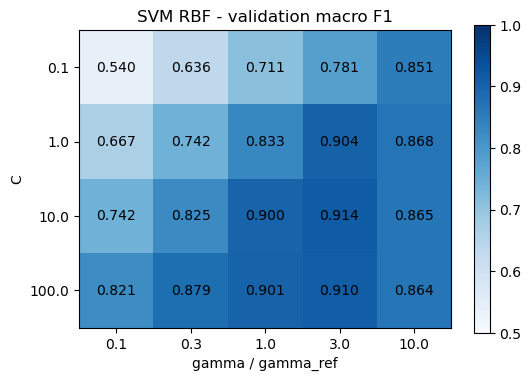
\includegraphics[width=\linewidth]
                {Images/SVM/svm_heatmap_validation.png}\\
            (a) Grid search
        \end{minipage}
        \hfill
        \begin{minipage}{0.44\linewidth}
            \centering
            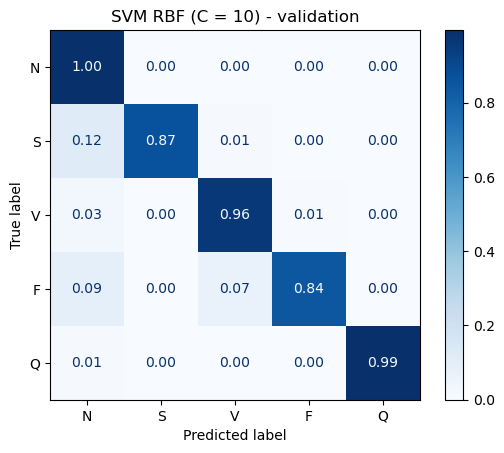
\includegraphics[width=\linewidth]
                {Images/SVM/svm_confusion_validation.png}\\
            (b) Selected model
        \end{minipage}
        \caption{RBF SVM on the validation set. (a) Macro F1 for
        each combination of $C$ and $\gamma$, trained on the 20\%
        subset. (b) Row-normalized confusion matrix of the selected
        model ($C = 10$, $\gamma = 3\gamma_{\mathrm{ref}}$), trained
        on the full training set.}
        \label{fig:svm_results}
    \end{figure}

    Figure~\ref{fig:svm_results}a shows the validation macro F1 of
    the grid. With small $C$ and $\gamma$ the score is 0.540, the
    same as logistic regression: with a wide kernel, the SVM behaves
    almost like a linear model. The score increases with $\gamma$
    up to $3\gamma_{\mathrm{ref}}$. At $10\gamma_{\mathrm{ref}}$ the
    training macro F1 reaches 1 for $C \geq 10$, while the
    validation score drops to about 0.865, so the model overfits.
    The best combination, $C = 10$ and
    $\gamma = 3\gamma_{\mathrm{ref}} = 0.0232$, lies inside the grid.

    Retrained on the full training set, the selected model reaches
    a training macro F1 of 0.982 and a validation macro F1 of
    0.939, higher than the 0.914 obtained on the subset. Compared with logistic regression, the main
    difference is on class N: its recall increases from 0.73 to
    0.996, so almost no normal beats are flagged as arrhythmias.
    As a consequence, the F1 of the minority classes improves
    considerably, from 0.33 to 0.89 for S and from 0.18 to 0.85
    for F.

    \subsection{Fully connected neural networks}

    We implemented multilayer perceptrons (MLPs) using
    \texttt{MLPClassifier} from scikit-learn~\cite{sklearn_docs} to learn nonlinear
    relationships between heartbeat features and the five AAMI
    classes. The initial configuration used the 250 raw signal
    samples as inputs and two fully connected hidden layers
    of 100 neurons each.
    \begin{figure}[htbp]
        \centering
        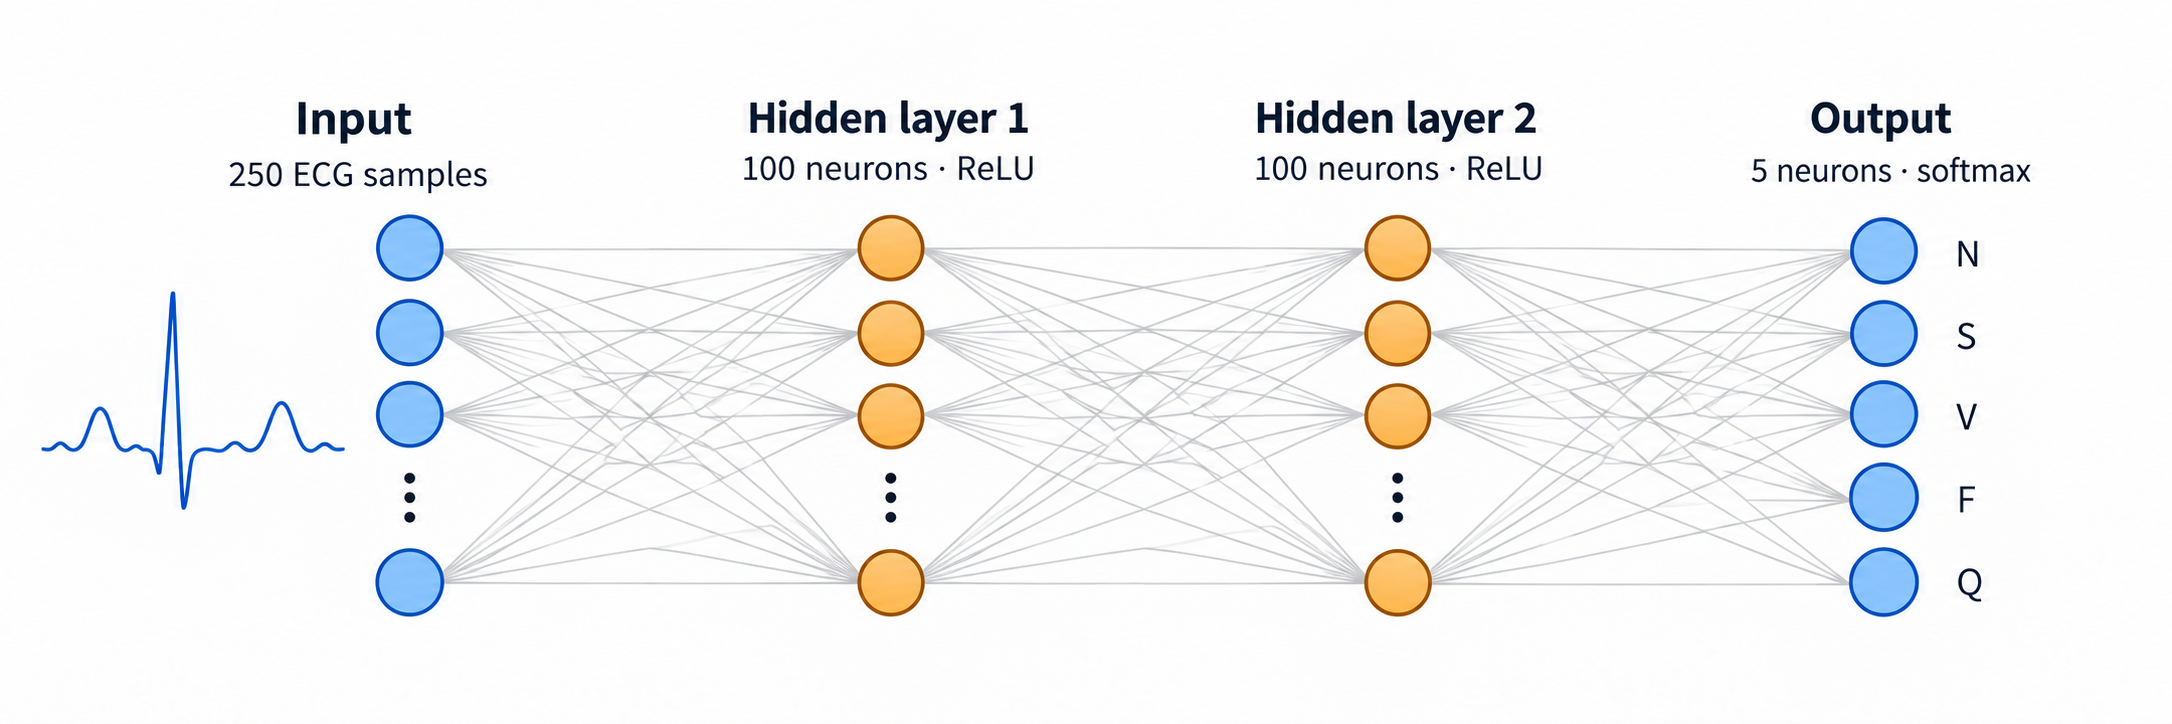
\includegraphics[width=\linewidth,trim=0 97bp 0 90bp,clip]
            {Images/mlp_architecture_generated.png}
        \caption{Selected MLP architecture for classification
        of raw ECG heartbeats.}
        \label{fig:mlp_architecture}
    \end{figure}
    All configurations used ReLU hidden-layer activations,
    the Adam optimizer and a maximum of 200 training epochs.
    We fixed \texttt{random\_state=42} for reproducibility.
    Training could terminate before this limit when the training
    loss no longer improved sufficiently, and this is what happened all the times.

    Hyperparameter tuning consisted of targeted comparisons
    using validation macro F1. We tested one, two and three
    hidden layers with 100 neurons per layer. For the two-layer
    architecture, we also tested 50 and 200 neurons per layer.
    The L2 regularization coefficient $\alpha$ was increased
    from $10^{-4}$ to $10^{-3}$ to assess whether stronger
    regularization improved generalization.

    The best tested configuration remained the initial
    two-layer network with 100 neurons per layer and
    $\alpha=10^{-4}$, achieving a validation macro F1 of 0.9375
    after 156 training epochs. This architecture was also
    evaluated with standardized, PCA and FFT features.
    None of the tested preprocessing configurations improved
    upon its performance on raw signals.
    \subsection{Convolutional neural networks}

    We implemented a one-dimensional CNN using
    TensorFlow/Keras~\cite{tensorflow_docs}
    to investigate whether learning local waveform patterns could
    improve heartbeat classification. Raw signals were reshaped
    into sequences of 250 samples with one input channel.
    Convolutional filters and classification layers are trained
    jointly~\cite{bronstein2021}.

    The architecture contains two convolutional layers with
    16 and 32 filters, respectively, kernel size 5, ReLU activation
    and same padding. Each convolutional layer is followed by
    max pooling with pool size 2. The resulting feature maps
    are flattened and passed to a fully connected layer with
    64 ReLU neurons, followed by five softmax output neurons.

    Training used Adam with learning rate $10^{-3}$,
    sparse categorical cross-entropy loss and batches of 128
    heartbeats, for a maximum of 50 epochs.
    Early stopping monitored validation loss with a patience
    of five epochs and restored the weights corresponding
    to its minimum.

    We compared the initial architecture with a variant adding
    dropout at rate 0.3 after the hidden dense layer, and a
    separate variant adding a second dense layer of 64 neurons.
    Configurations were selected using validation macro F1.
    The dropout variant achieved the best CNN score of 0.9273,
    remaining below the 0.9375 obtained by the selected MLP.
    \begin{figure}[H]
        \centering
        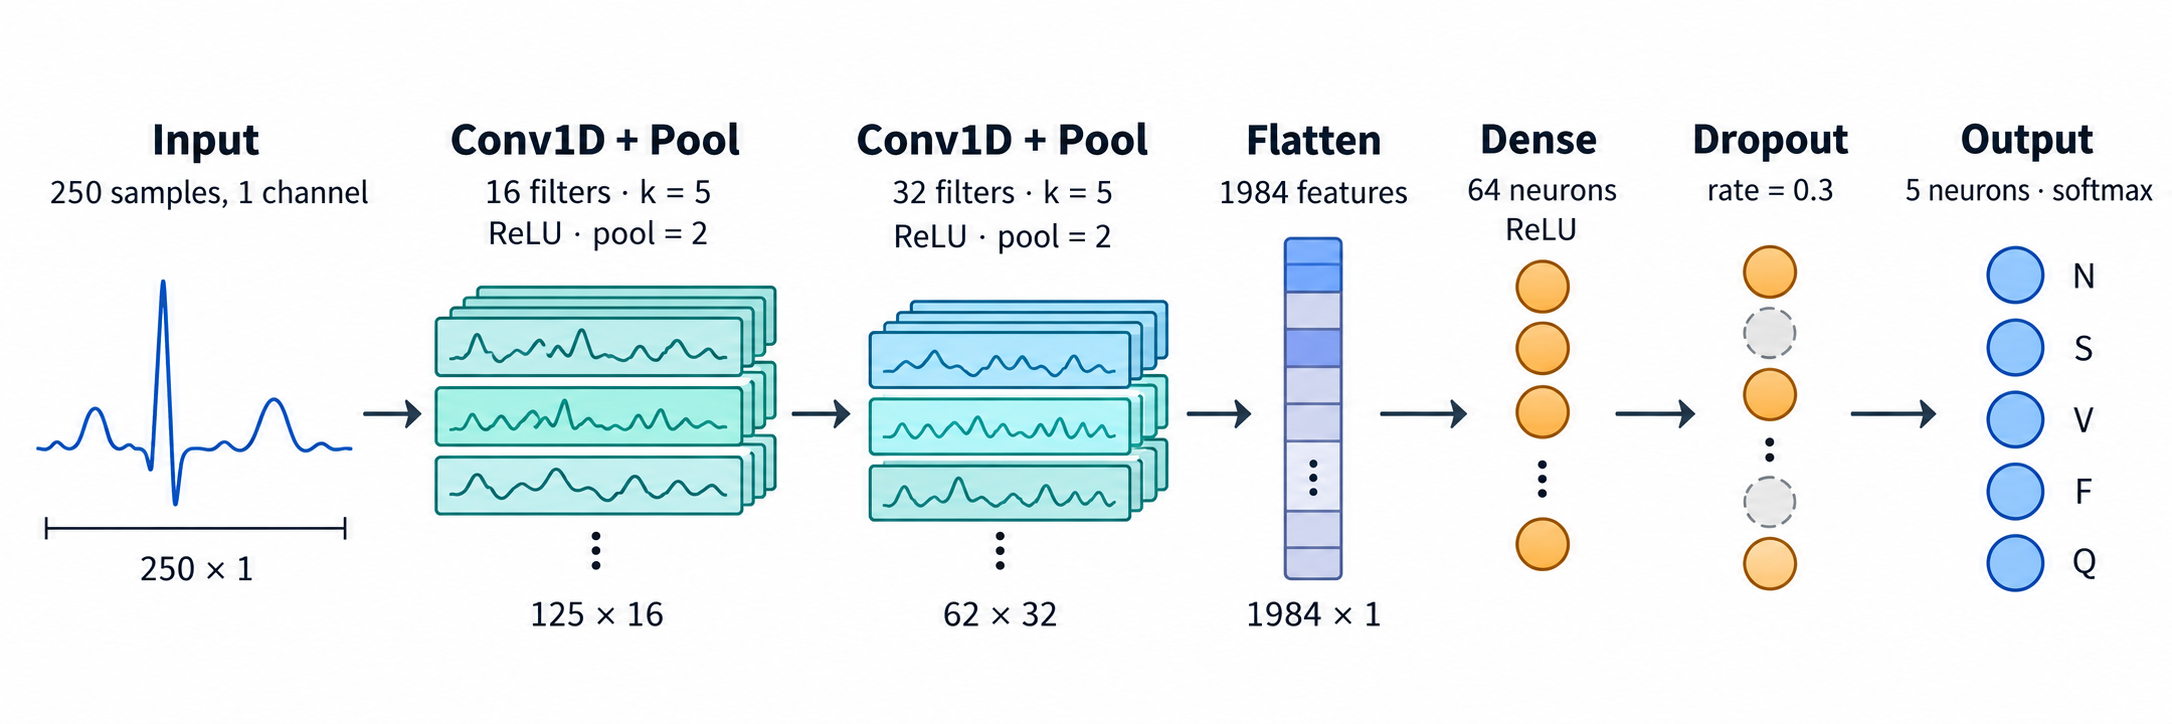
\includegraphics[width=\linewidth,trim=0 88bp 0 112bp,clip]
            {Images/cnn_architecture_generated.png}
        \caption{Selected CNN architecture for raw ECG
        classification. Each convolutional block includes
        ReLU activation and max pooling; $k$ denotes
        the kernel size.}
        \label{fig:cnn_architecture}
    \end{figure}
    \section{Results and Discussion}
    \subsection{Validation results and hyperparameter selection}
    We compared 108 candidate configurations: 72 for logistic
    regression, 20 for RBF SVM, 13 for MLP and three for CNN.
    Preprocessing and hyperparameters were compared using macro F1
    on the supplied validation set. SVM tuning used a stratified
    20\% subset of the training data; the selected configuration
    was then fitted on the full training set.
    Table~\ref{tab:validation_comparison} compares the best tested
    configurations with the majority baseline.

    \begin{table}[htbp]
        \centering
        \begin{tabular}{@{}p{0.23\linewidth}p{0.52\linewidth}r@{}}
            \toprule
            Model & Selected input representation & Val.\ macro F1 \\
            \midrule
            Majority baseline
                & --
                & 0.181 \\
            Logistic regression
                & Per-beat normalization
                & 0.554 \\
            RBF SVM
                & Per-beat normalization + PCA (100 components)
                & 0.939 \\
            MLP
                & Raw signals
                & 0.9375 \\
            CNN with dropout
                & Raw signals
                & 0.9273 \\
            \bottomrule
        \end{tabular}
        \caption{Validation performance of the baseline and the
        best tested configuration of each classifier.}
        \label{tab:validation_comparison}
    \end{table}
    The selected SVM, MLP and CNN substantially outperformed
    logistic regression and were retained for final test evaluation.
    \subsection{Final test results and error analysis}

    The configurations selected using validation macro F1 were
    evaluated on the test set. Table~\ref{tab:test_comparison}
    reports their final performance. The ordering observed on
    validation was preserved, with the SVM achieving the highest
    test macro F1, followed by the MLP and CNN. All three models
    obtained slightly lower macro F1 than on validation.

    \begin{table}[htbp]
        \centering
        \begin{tabular}{lrrrrr}
            \toprule
            Model & Accuracy & Macro P & Macro R
                & Macro F1 & Weighted F1 \\
            \midrule
            SVM & 0.988  & 0.940  & 0.929
                & 0.935  & 0.988 \\
            MLP & 0.9864 & 0.9251 & 0.9301
                & 0.9275 & 0.9865 \\
            CNN & 0.9854 & 0.9622 & 0.8761
                & 0.9134 & 0.9848 \\
            \bottomrule
        \end{tabular}
        \caption{Final test results for the selected configurations.
        P and R denote precision and recall.}
        \label{tab:test_comparison}
    \end{table}

    Accuracy exceeded 98.5\% for every model, while macro F1
    revealed larger differences. This reflects the strong class
    imbalance: reliable classification of the majority class can
    coexist with poorer recognition of minority classes.

    Table~\ref{tab:test_per_class} shows the per-class F1 scores.
    All models performed well on N, V and Q, while S and F
    remained more difficult. The SVM's advantage over the MLP
    was most evident on S. Its precision for this class was
    0.895, compared with 0.851 for the MLP, while their recalls
    were similar, at 0.888 and 0.892, respectively. On F, their
    F1 scores were almost identical.

    \begin{table}[htbp]
        \centering
        \begin{tabular}{lrrrrr}
            \toprule
            Model & N & S & V & F & Q \\
            \midrule
            SVM & 0.994  & 0.892  & 0.973
                & 0.820  & 0.994 \\
            MLP & 0.9930 & 0.8709 & 0.9605
                & 0.8190 & 0.9938 \\
            CNN & 0.9920 & 0.8253 & 0.9682
                & 0.7885 & 0.9928 \\
            \bottomrule
        \end{tabular}
        \caption{Test F1 scores for each AAMI class.}
        \label{tab:test_per_class}
    \end{table}

    \begin{figure}[htbp]
        \centering
        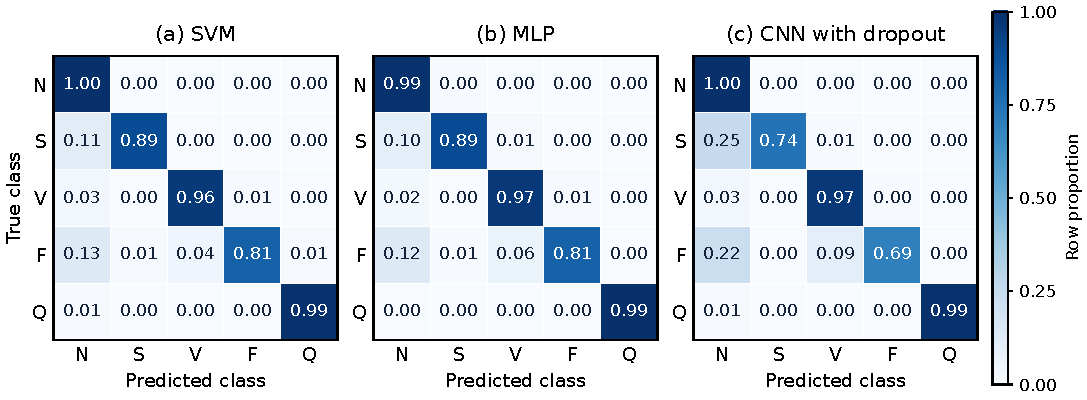
\includegraphics[width=\linewidth]
            {Images/Results/test_confusion_matrices.pdf}
        \caption{Row-normalized test confusion matrices for the
        selected SVM, MLP and CNN. Rows represent true classes
        and columns predicted classes. Values are proportions,
        rounded to two decimal places.}
        \label{fig:test_confusion_matrices}
    \end{figure}

    Figure~\ref{fig:test_confusion_matrices} shows the
    distribution of classification errors.
    The CNN combined high macro precision with lower macro
    recall, particularly for S and F. It correctly identified
    73.9\% of S beats and 68.8\% of F beats. Its confusion matrix
    shows that 141 of the 556 S beats were classified as N.
    Among the 160 F beats, 35 were classified as N and 15 as V.
    These errors explain why its high overall accuracy did not
    translate into equally strong performance across all classes.
    \subsection{Additional experiment: 15-class classification}

    We retrained the selected raw-signal MLP on the original
    15 labels, retaining the same architecture and hyperparameters.
    Validation accuracy was 98.47\%, with a macro F1 of 0.7140
    across all 15 labels.

    Label 9 has only two training examples and none in validation,
    so its generalization performance could not be assessed.
    This absent class contributes an F1 of zero to the reported
    15-class average. Restricting the average to the 14 classes
    present in validation gives a macro F1 of 0.7650.

    Labels 4 and 14 had only three and six validation examples,
    respectively, and no correct predictions. Their zero F1
    scores show how overall accuracy can conceal poor recognition
    of rare classes.

    \subsection{Limitations}

    Experiments used the supplied fixed splits and a single
    random seed. Variability across data splits and neural network
    initializations was therefore not quantified, and small
    performance differences should be interpreted cautiously.

    Class imbalance also limits the reliability of per-class
    estimates. For example, class F contains only 160 test beats,
    making its results sensitive to a small number of predictions.
    High aggregate scores consequently provide limited evidence
    of reliable recognition of every heartbeat type.

    Hyperparameter searches covered finite grids and selected
    neural network architectures, with different search spaces
    for each model family. The SVM grid additionally used only
    20\% of the training data, so the selected parameters might
    differ from those preferred when tuning on the full training
    set. Our conclusions apply to the tested configurations
    and search spaces.

    \section{Conclusions}

    We compared logistic regression, RBF SVM, MLP and CNN models
    for ECG heartbeat classification into five AAMI classes,
    selecting configurations using validation macro F1.

    The selected SVM achieved the highest test macro F1,
    approximately 0.935, followed by the raw-signal MLP at 0.9275
    and the CNN at 0.9134. The MLP used two hidden layers of
    100 neurons. Among the tested architectures, convolutional
    layers and greater network complexity did not improve upon
    this configuration.

    Preprocessing choices depended on the classifier. The
    selected SVM used per-beat normalization and 100 PCA
    components, while raw signals remained the best MLP input.
    Real and imaginary FFT features gave similar validation
    performance to raw signals; magnitude-only features reduced
    dimensionality at the cost of lower macro F1.

    Recognition of S and F remained challenging. The additional
    15-class experiment further showed how high accuracy can
    conceal poor recognition of rare heartbeat types.
    Further work could quantify variability across random seeds
    and explore a broader range of CNN architectures.

    \begin{thebibliography}{9}
        \small
        \raggedright

        \bibitem{course_materials}
        TU Delft.
        \emph{EE4C12: Machine Learning for Electrical Engineering
        Applications}. Course lecture slides and code labs,
        including Feature Engineering and Learning, Neural Networks,
        and Machine Learning Workflow.

        \bibitem{sklearn_docs}
        scikit-learn developers.
        \emph{scikit-learn documentation: User Guide and API Reference}.
        \url{https://scikit-learn.org/stable/}.
        Accessed 9 October 2026.

        \bibitem{tensorflow_docs}
        TensorFlow developers.
        \emph{TensorFlow documentation: Keras API}.
        \url{https://www.tensorflow.org/api_docs/python/tf/keras}.
        Accessed 4 October 2026.

        \bibitem{bronstein2021}
        M.~M. Bronstein, J. Bruna, T. Cohen, and P. Veli\v{c}kovi\'{c}.
        \emph{Geometric Deep Learning: Grids, Groups, Graphs,
        Geodesics, and Gauges}. arXiv:2104.13478, 2021,
        Sections 4.2 and 5.1.
        \url{https://arxiv.org/abs/2104.13478}.
    \end{thebibliography}

    {\small
    \noindent\textbf{Use of AI.}
    ChatGPT was used to support report
    drafting and summarization, help organize the results, and assist with writing and debugging
    selected Python notebook cells. AI was also used to create the NN and CNN
    architecture diagrams and adapt the layout of the PCA variance plot.
    The authors are responsible for the final content, analyses
    and conclusions.\par}

\end{document}
